In this section, we outline the benchmarking results employed from the methodologies.
We benchmark the DON framework with Pixelwise NT-Xent loss as in \cite{adrian2022efficient} and our framework
with our revision of the loss function on a 48GB VRAM GPU. We benchmark the descriptor's robustness
with the $AUC \pm \sigma$ for $PCK@k, \forall k \in [1, 100]$ metric.
Furthermore, we benchmark the computational resource consumption of the DON and our frameworks.
We also demonstrate the application of our framework as a robot-grasping pipeline in two methodologies,
one of which our framework demonstrates its capabilities to produce object-specific 6D poses for robot grasping.


\subsection{Training Setup}
We implemented training and benchmarking using ``PyTorch-Lightning''\cite{falcon2019pytorch} and ``PyTorch''\cite{paszke2019pytorch} libraries.
Furthermore, we employ
ADAM\cite{kingma2014adam} optimizer to optimize the model for 2500 epochs with a learning rate of
$\alpha = 3 \times 10^{-4}, \beta_1 = 0.9 \text{ and } \beta_2 = 0.999$ with weight decay $\eta =10^{-4}$ to benchmark the DON with Pixelwise NT-Xent loss as in ~\cite{adrian2022efficient}
with a fixed batch size of 1 and 128 image-pair correspondences.

To train our framework, we employ an ADAM optimizer to optimize the model for 2500 epochs with a learning rate of
$\alpha = 1 \times 10^{-3}, \beta_1 = 0.9 \text{ and } \beta_2 = 0.999$ with no weight decay.
We further use a fixed batch size of 1 and the StepLR scheduler with a step size 2500 and a gamma of 0.9 to train the model with all the loss weights to $1.0$ except variance loss weight to $1 \times 10^{-3}$.
We trained the three models with 128 keypoints with a margin of 2 pixels for each descriptor dimension. We specifically chose 128 keypoints as it aligns with the notion that DON is benchmarked with 128 image-pair correspondences.

\subsection{Benchmarking \& Results}
The $AUC \pm \sigma$ for $PCK@k, \forall k \in [1, 100]$ is computed with 256 image-pair correspondences for both models.
The metrics mean and std. deviation is calculated from benchmarking three models trained for each descriptor dimension.
Due to the limited GPU VRAM capacity, we could not train DON for descriptor dimensions greater than 32.
As per Table~\ref{table:benchmark_auc}, both frameworks benefit while training them for longer descriptor dimensions.
Furthermore, the higher values infer robust descriptors in Table~\ref{table:benchmark_auc}. We notice that our framework
works robustly as the descriptor dimension gets longer as the metric difference between DON and our framework reduces.

\begin{table}[htb]
    \caption{Benchmarking outcomes for descriptors' evaluation metric.}
    \centering
    \label{table:benchmark_auc}
    \begin{tabular}{ccc}
        \toprule
        \multicolumn{3}{c}{Benchmarking for $AUC \pm \sigma$ for $PCK@k, \forall k \in [1, 100]$} \\
        \midrule
        Descriptor Size ($D$) & Dense Object Nets          & Our framework                        \\ \hline
        3                     & $\mathbf{0.922 \pm 0.006}$ & $0.914 \pm 0.009$                    \\
        8                     & $\mathbf{0.933 \pm 0.011}$ & $0.928 \pm 0.015$                    \\
        16                    & $\mathbf{0.948 \pm 0.012}$ & $0.945 \pm 0.010$                    \\
        32                    & $\mathbf{0.953 \pm 0.008}$ & $0.950 \pm 0.009$                    \\
        64                    & $ \mathtt{\sim}$           & $0.953 \pm 0.006$                    \\
        128                   & $ \mathtt{\sim}$           & $0.957 \pm 0.012$                    \\
        256                   & $ \mathtt{\sim}$           & $0.959 \pm 0.008$                    \\
        512                   & $ \mathtt{\sim}$           & $0.962 \pm 0.011$                    \\
        \bottomrule
    \end{tabular}
\end{table}

While training both frameworks, we monitor the GPU VRAM consumption.
As per the benchmark results in Table~\ref{table:benchmark_gpu},
the DON consumption increases as the descriptor dimensions get longer while our
framework consumes a fraction of the computation resource.
Furthermore, lower readings are better in Table~\ref{table:benchmark_gpu}.

\begin{table}[htb]
    \caption{Benchmarking outcomes for training computation resource comsumption.}
    \label{table:benchmark_gpu}
    \centering
    \begin{tabular}{ccc}
        \toprule
        \multicolumn{3}{c}{Benchmarking for GPU VRAM(GB) consumption} \\
        \midrule
        Descriptor Size ($D$) & Dense Object Nets & Our framework     \\ \hline
        3                     & $9.377$           & $\mathbf{4.763}$  \\
        8                     & $13.717$          & $\mathbf{4.785} $ \\
        16                    & $20.479$          & $\mathbf{4.832} $ \\
        32                    & $30.067$          & $\mathbf{4.872} $ \\
        64                    & $ \mathtt{\sim}$  & $4.913$           \\
        128                   & $ \mathtt{\sim}$  & $5.409 $          \\
        256                   & $ \mathtt{\sim}$  & $6.551 $          \\
        512                   & $ \mathtt{\sim}$  & $7.915 $          \\
        \bottomrule
    \end{tabular}
\end{table}

To check the impact of descriptors' robustness compared to the number of keypoints, we trained our framework with 16 keypoints.
Furthermore, we trained three additional models for each descriptor dimension 64, 128, 256, and 512.
As per the Table~\ref{table:reduced_framework_training_results} compared to the results in Table~\ref{table:benchmark_auc} in page~\ref{table:benchmark_auc},
the descriptor's robustness decreased when the framework predicted 16 keypoints.
Moreover, this reflects that number of keypoints in our framework and the number of image-pair correspondences in DON are directly proportional to the robustness of the descriptors.


\begin{table}[htb]
    \caption{Benchmark of our framework with 16 keypoints for GPU VRAM(GB) consumption and $AUC \pm \sigma$ for $PCK@k,  \forall k \in [1, 100]$ metric.}
    \label{table:reduced_framework_training_results}
    \centering
    \begin{tabular}{ccc}
        \toprule
        \multicolumn{3}{c}{Our framework with 16 keypoints}         \\
        \midrule
        Descriptor Size ($D$) & Metric            & VRAM Usage (GB) \\ \hline
        64                    & $0.948 \pm 0.009$ & $3.799 $        \\
        128                   & $0.952 \pm 0.010$ & $4.191 $        \\
        256                   & $0.955 \pm 0.013$ & $5.241 $        \\
        512                   & $0.957 \pm 0.006$ & $7.341 $        \\
        \bottomrule
    \end{tabular}
\end{table}

\subsection{Descriptor Inspection}
Furthermore, to inspect the
results of trained DON, an interface is built using the PyGame library~\cite{pygame} to visualize the results of the trained DON.
The mouse pointer in the image space is mapped to the pixel, and the descriptor at that pixel is queried in another image-descriptor space.
We further use the spatial probability of the descriptor to visualize the queried descriptor
in the image space using Equation~\ref{eqn:gaussian_kernel} in page~\pageref{eqn:gaussian_kernel}.
We identify if there are any multi-modal spatial activations in the descriptor spaces and none, as shown in Figure~\ref{fig:check_don}.

\begin{figure}[htb]
    \centering
    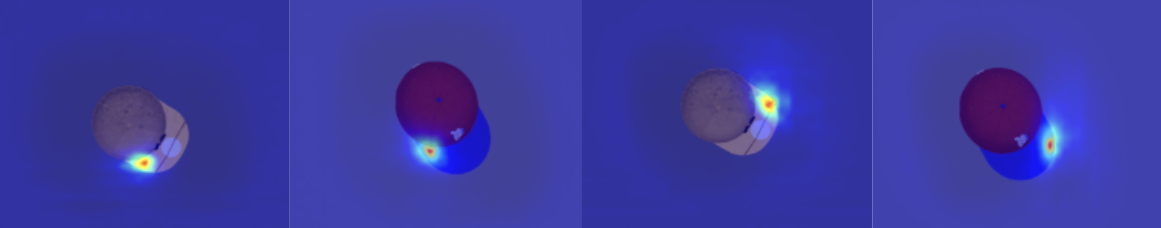
\includegraphics[scale=0.15]{../images/test_don.png}
    \caption{Depiction of the spatial probability heatmaps of the descriptor in the image space. We set the temperature in the Equation~\ref{eqn:gaussian_kernel} to $1.1$
        and render the spatial probability heatmaps in the interface. The first and second image from the left and the right highlights the semantically equivalent descriptors in the image space.}
    \label{fig:check_don}
\end{figure}

For the robot grasping pipeline, we trained our framework with actual caps.
As the synthetic data generation only needs mask and depth information, we could create a mask in no time.
Additionally, while training the framework, we do not need the actual real-world depth information as it computes its own.
We later extracted the dense visual local descriptors from the framework.
We visually inspected for any inconsistencies in the descriptor space, as shown in Figure~\ref{fig:check_real_caps},
and found it consistent. Furthermore, we did not use the models trained on the synthetic dataset, as the representations were inconsistent with the real caps.

\begin{figure}[htb]
    \centering
    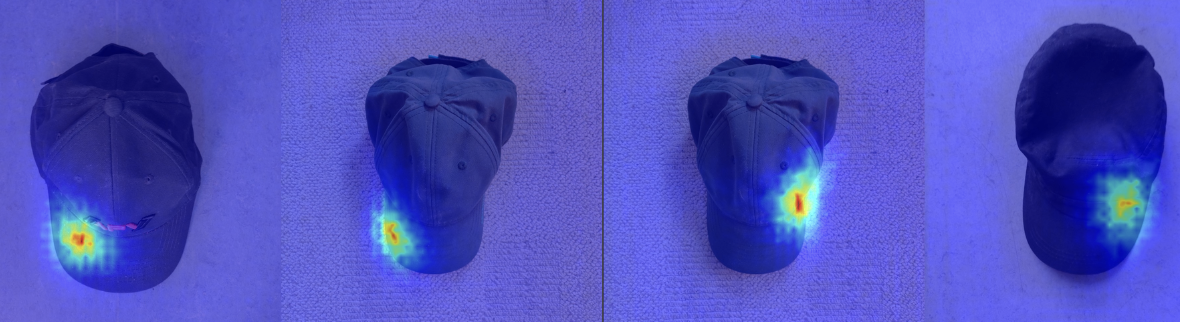
\includegraphics[scale=0.125]{../images/test_real_caps.png}
    \caption{The image depicts the visual inspection of the dense visual descriptors space of the real caps using our developed interface. We trained our framework on the first two caps from the left, and our framework could generalize the object representations on an unseen cap while training illustrated in the first image from the right.}
    \label{fig:check_real_caps}
\end{figure}



\subsection{Robot Grasping Pipeline}

For robot grasping, a descriptor is picked from the descriptor space and queried in real-time such that robot can pinch-grasp the object.
We could successfully grasp the caps with the robot, as shown in Figure~\ref{fig:straight_grasp}.
Furthermore, we did not evaluate the robot grasping for position and semantic object location offsets.

\begin{figure}[htb]
    \centering
    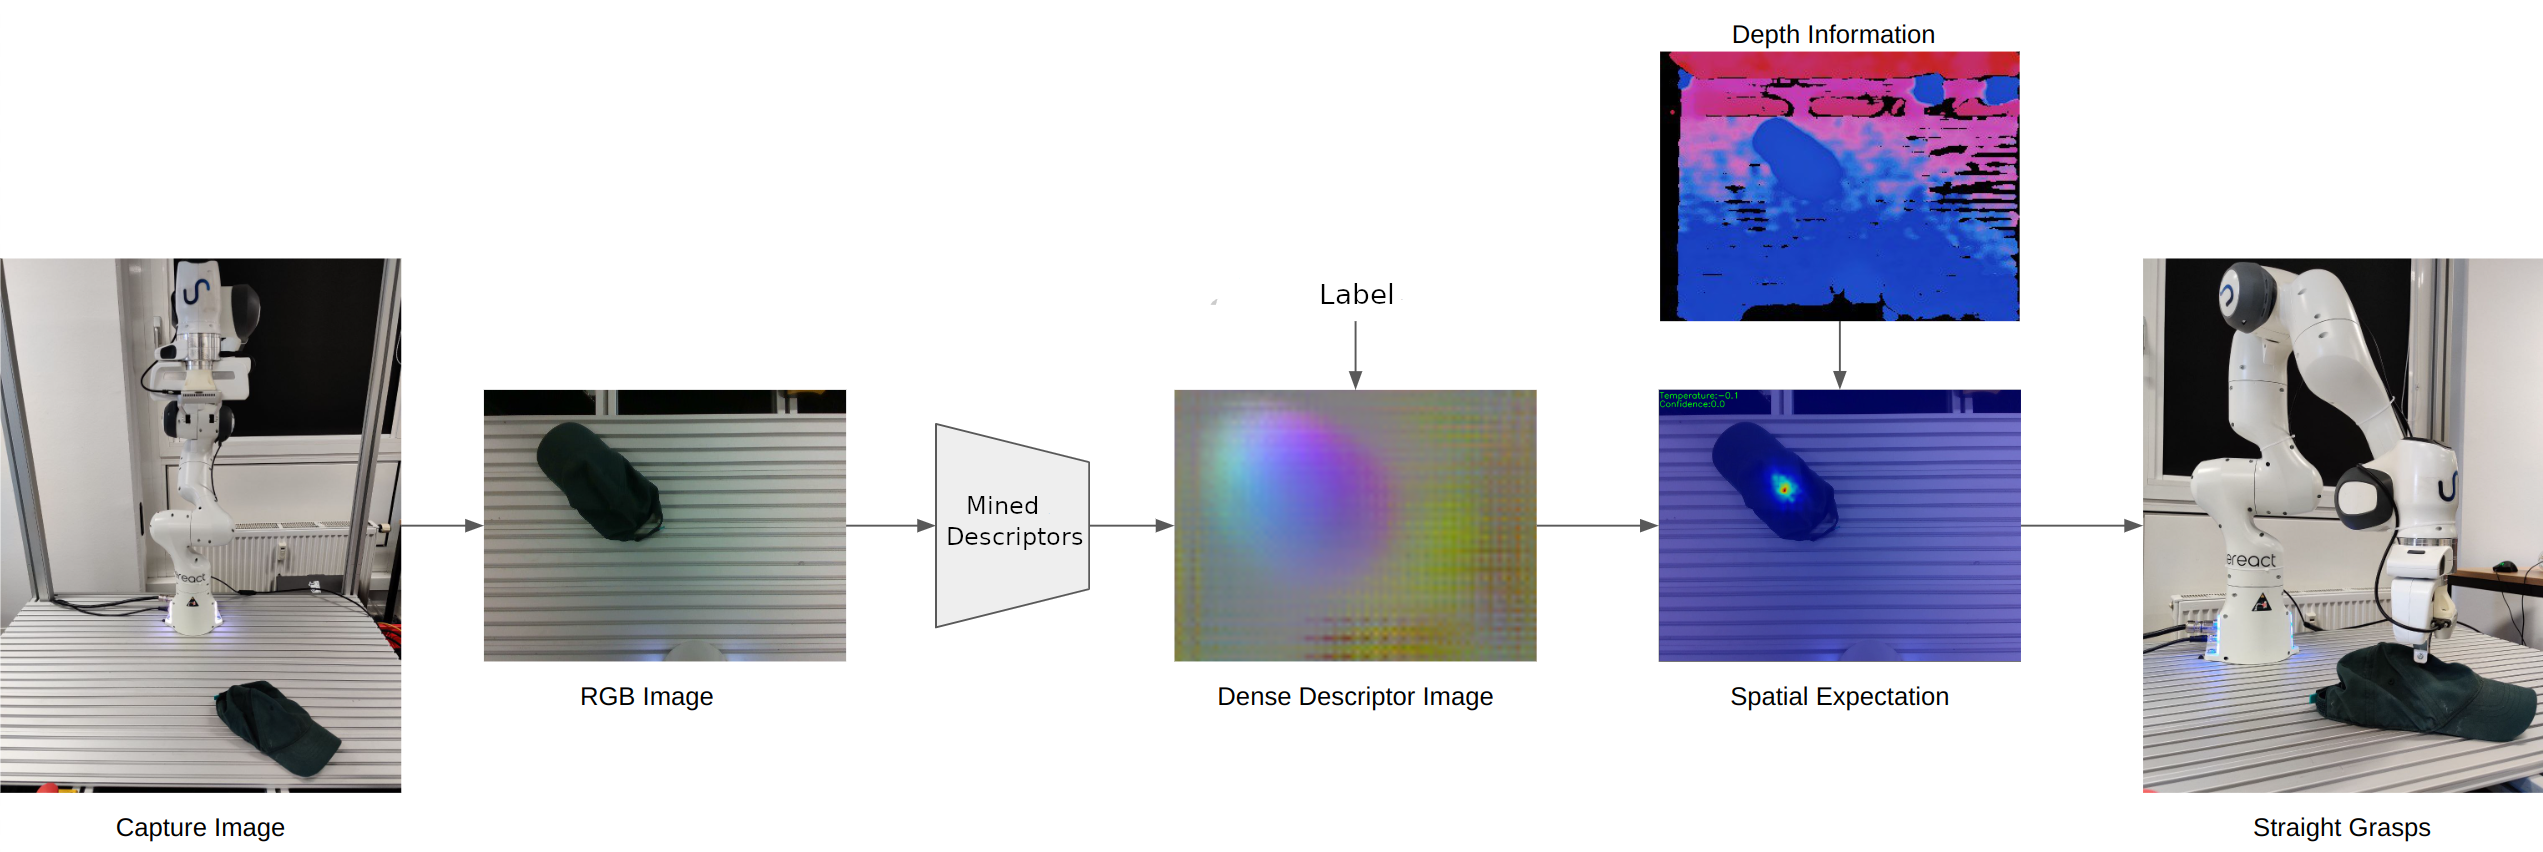
\includegraphics[scale=0.1]{../images/straight_grasps.png}
    \caption{Depiction of the straight robot grasping pipeline.}
    \label{fig:straight_grasp}
\end{figure}

As our framework inertly regresses keypoints on the object, we could use it as an alternative approach to grasp the caps by computing the pose
generated by the keypoints considering the actual depth information instead of network-regressed depth information.
We extract the spatial probability of each keypoint from the framework and deactivate spatial probabilities where the depth information is missing,
as the depth image from the camera is noisy. Furthermore, the spatial expectations of the keypoints are projected to the camera frame
to calculate a 6D pose in the camera frame. The 6D pose is transformed in the robot frame to perform an aligned grasp, as shown in Figure~\ref{fig:aligned_grasp}.

\begin{figure}[htb]
    \centering
    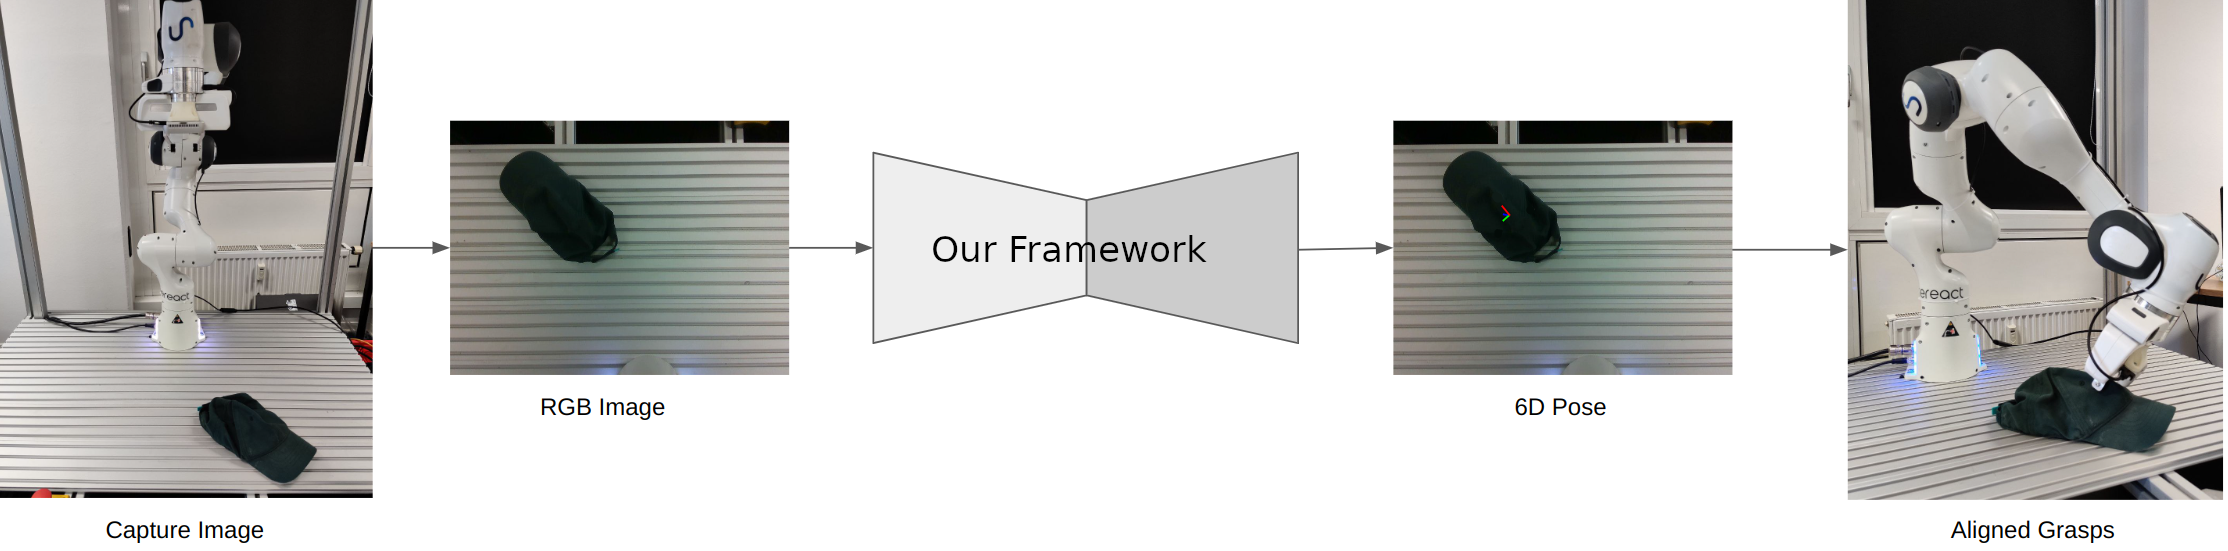
\includegraphics[scale=0.15]{../images/aligned.png}
    \caption{Illustration of the aligned robot grasping pipeline.}
    \label{fig:aligned_grasp}
\end{figure}

